\documentclass[12bp]{guo}
\usepackage{guo}
\usepackage{minted}
\usepackage{titlesec}
\usepackage{indentfirst}
\usepackage[labelformat=empty]{caption}

% source code listing
\usemintedstyle{vs}

% title
\titleformat
{\section}
[block]
{\fontlf}
{}
{0ex}
{}
[]
\setcounter{section}{0}

\titleformat
{\subsection}
[block]
{\fontli}
{}
{0ex}
{}
[]
\setcounter{subsection}{0}

\titleformat
{\subsubsection}
[block]
{\fontlj}
{}
{0ex}
{}
[]
\setcounter{subsubsection}{0}

% fixup reference title
\renewcommand\refname{}

% figure
\renewcommand{\figurename}{}
\renewcommand{\thefigure}{}

\begin{document}

\section{一、设计目的}

本课程设计要求设计一个模拟的多用户多级目录的文件系统。
通过具体的文件存储空间的管理、文件的物理结构、目录结构和文件操作的实现,
加深对文件系统内部功能和实现过程的理解。

\section{二、设计内容}

\begin{description}
    \item{(1)} 在内存中开辟一个虚拟磁盘空间作为文件存储器,
               在其上实现一个多用户多目录的文件系统。
               
    \item{(2)} 文件物理结构可采用连续结构。 
        
    \item{(3)} 磁盘空闲空间的管理选择位示图。 
        
    \item{(4)} 文件目录结构采用多用户多级目录结构,每个目录项包含文件名、
               物理地址、长度等信息,还可以通过目录项实现对文件的读和写的保护。 
               
    \item{(5)} 设计一个较实用的用户界面,方便用户使用。要求提供以下相关文件操作: 
        
        \begin{description}
            \item{(1)} 具有login (用户登录) 
            \item{(2)} 系统初始化(建文件卷、提供登录模块)
            \item{(3)} 文件的创建: create 
            \item{(4)} 文件的打开:open
            \item{(5)} 文件的读:read
            \item{(6)} 文件的写:write
            \item{(7)} 文件关闭:close
            \item{(8)} 删除文件:delete
            \item{(9)} 创建目录(建立子目录):mkdir
            \item{(10)} 改变当前目录:cd
            \item{(11)} 列出文件目录:dir
            \item{(12)} 退出:logout
        \end{description}
\end{description}

\section{三、设计步骤}

\subsection{需求分析}

本课程设计需要提供一个简单易用的界面来管理文件系统,并通过一系列操作来和
该文件系统进行交互。


文件系统本身记录保存在内存中;系统物理结构采用连续记录方式,即所有文件记录按照
一定顺序连续写入到内存中。为了方便检索,文件系统通过位示图来记录物理结构中的空闲区块。


而系统也需要提供简单的权限控制来保护文件,方便处理多用户下的协作。

\subsection{概要设计}

通过需求分析可以知道,需要将系统划分以下三个模块:

\begin{description}
    \item{交互管理模块} 该模块主要负责处理用户的输入(例如键盘、鼠标),
                        并将操作转发到其他两个模块处。
    \item{用户管理模块} 该模块提供用户管理功能,例如登录、权限控制。
    \item{文件系统模块} 该模块负责实现文件系统,并且提供基本的文件管理功能。
\end{description}

这三个模块的关系如下图所示:

\begin{figure}[h!]
    \centering
        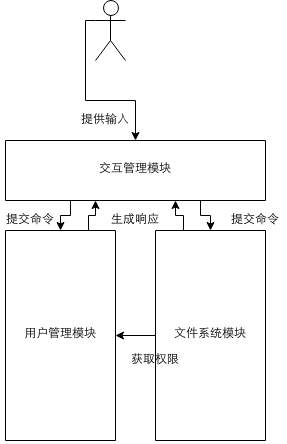
\includegraphics[scale=0.75]{figures/fs-app.module.png}
\end{figure}

\subsection{详细设计}

\subsubsection{实现途径}

程序运行在浏览器端,主要功能使用 typescript 和 css 来实现。

\subsubsection{功能定义}

根据需求分析,程序有以下几个功能:

\begin{description}
    \item{用户会话管理} 实现用户登录、退出等操作
    \item{文件的增删改} 针对文件的具体操作
    \item{文件的查询显示} 需要提供界面来查看文件系统中的目录情况
\end{description}

文件相关操作流程图如下:

\begin{figure}[h!]
    \centering
        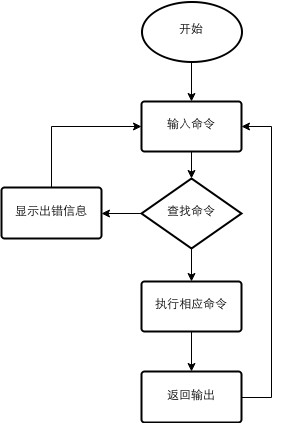
\includegraphics[scale=0.75]{figures/fs-app.flow.png}
\end{figure}



\subsection{调试分析}

由于系统运行在浏览器上,所以一刷新就会把原来的数据重置,这样会给调试带来很大的麻烦。
为了解决这个问题,我向程序添加了一个初始化模块,可以向其中指定一系列的初始化操作。
这样每次重新编译、刷新程序都可以保证有一个一致的初始状态,方便进行重复的调试。

\clearpage
\subsection{系统测试}

系统模块截图如下:

\begin{figure}[h!]
    \centering
        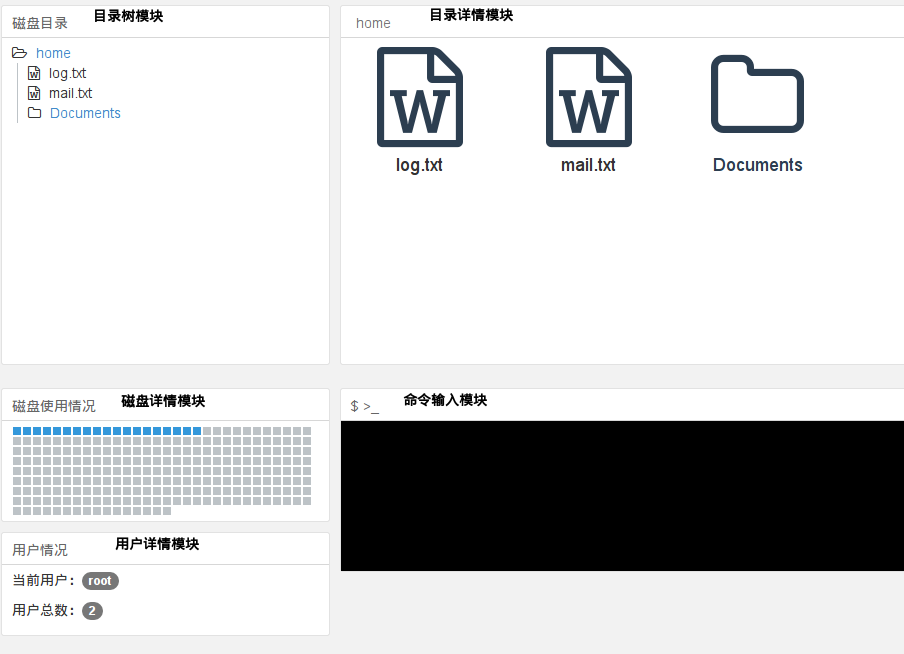
\includegraphics[scale=0.5]{figures/fs-app.overview.png}
\end{figure}

\clearpage

\subsubsection{用户会话管理}

可以通过 \mintinline{shell}{login} 和 \mintinline{shell}{logout} 命令来进行
登录、登出操作:

打开系统之后,会自动以 root 用户进行登录。可以通过 \mintinline{shell}{logout}
命令来进行登出操作,登出后需要再次登录才能继续进行操作:

\begin{figure}[h!]
    \centering
        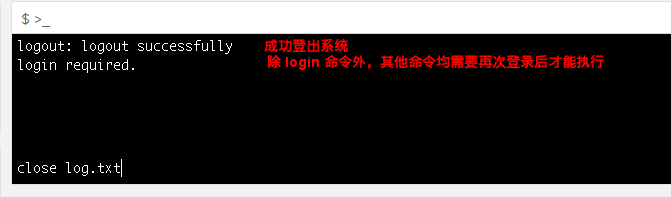
\includegraphics[scale=0.7]{figures/fs-app.logout.png}
\end{figure}


可以通过 \mintinline{shell}{login} 指令来再次登录:

\begin{figure}[h!]
    \centering
        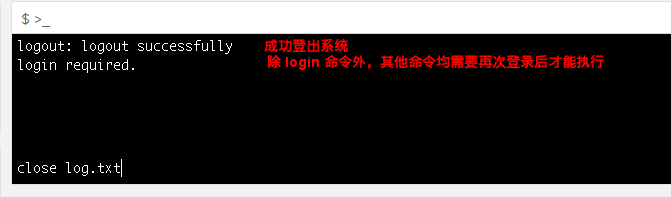
\includegraphics[scale=0.7]{figures/fs-app.logout.png}
\end{figure}


同时可以通过左侧的用户详情模块查看到当前登录用户身份:

\begin{figure}[h!]
    \centering
        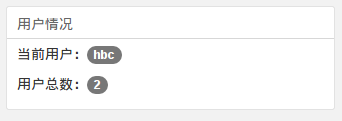
\includegraphics[scale=0.7]{figures/fs-app.user-stats.png}
\end{figure}

\clearpage

\subsubsection{文件增删改操作}

可以通过 \mintinline{shell}{open FILENAME} 的指令格式来打开一个文件,
打开成功后会显示对应文件描述符:

\begin{figure}[h!]
    \centering
        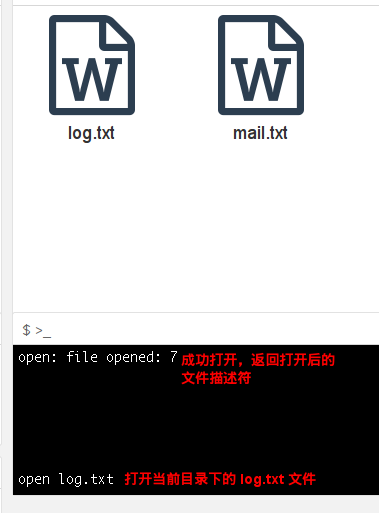
\includegraphics[scale=0.75]{figures/fs-app.open.png}
\end{figure}


成功打开之后可以对文件进行读取或写入操作:

\begin{figure}[h!]
    \centering
        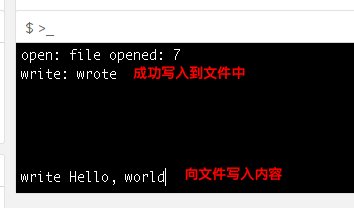
\includegraphics[scale=0.75]{figures/fs-app.write.png}
\end{figure}

\begin{figure}[h!]
    \centering
        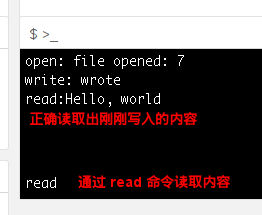
\includegraphics[scale=0.75]{figures/fs-app.read.png}
\end{figure}

并通过 \mintinline{shell}{close} 命令来关闭已经打开的文件。


而删除一个文件可以通过 \mintinline{shell}{rm} 来进行:

\begin{figure}[h!]
    \centering
        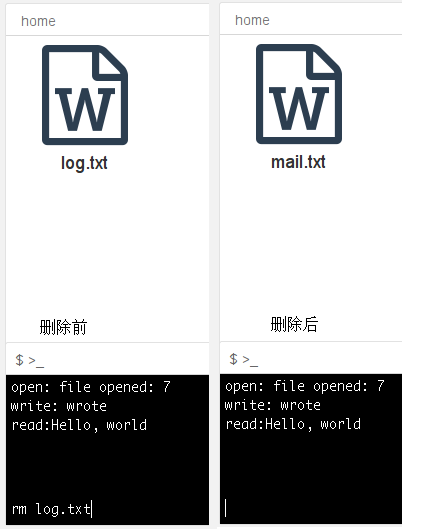
\includegraphics[scale=0.75]{figures/fs-app.rm-before.png}
\end{figure}

\clearpage

可以看到指定文件已被成功删除。而尝试删除其他用户的文件时,则会自动抛出错误,
禁止删除:

\begin{figure}[h!]
    \centering
        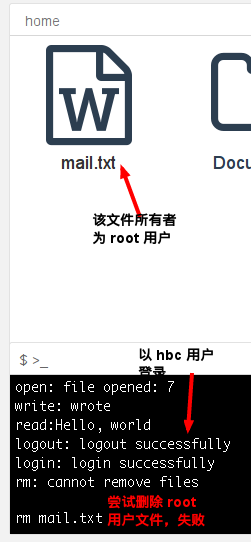
\includegraphics[scale=0.75]{figures/fs-app.rm-failed.png}
\end{figure}

从上面几个测试用例即可以看到系统按照预期正常工作。

\clearpage

\subsubsection{文件查询显示}

为了简化用户操作,文件系统详情可以直接在界面上显示出来:

1. 显示文件夹中的文件列表:

\begin{figure}[h!]
    \centering
        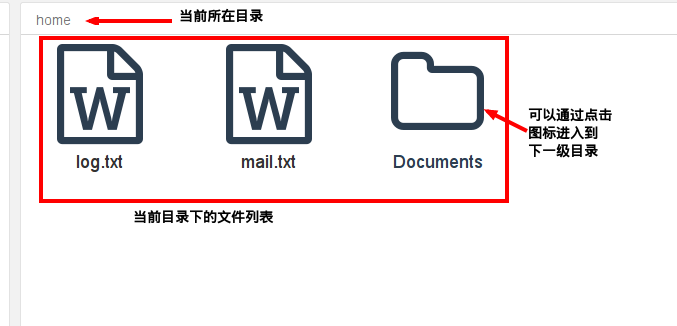
\includegraphics[scale=0.75]{figures/fs-app.list.png}
\end{figure}


2. 查看文件系统目录树:

用户可以通过左侧目录树来查看磁盘目录树。

\begin{figure}[h!]
    \centering
        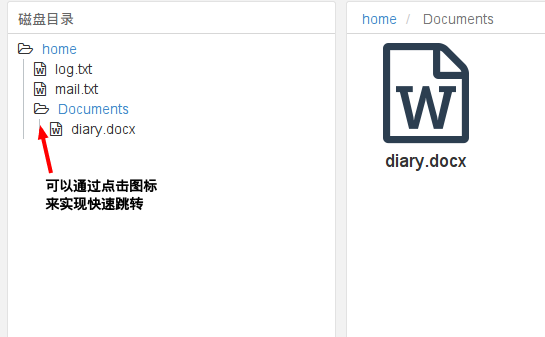
\includegraphics[scale=0.75]{figures/fs-app.tree.png}
\end{figure}


\clearpage
3. 查看磁盘使用情况:

\begin{figure}[h!]
    \centering
        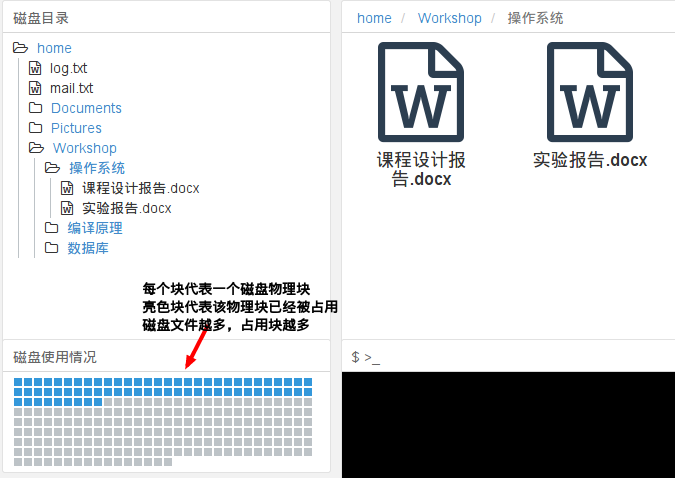
\includegraphics[scale=0.75]{figures/fs-app.disk.png}
\end{figure}


通过上述三个模块即可全面地了解到磁盘和目录使用情况。

\subsection{使用说明}

\begin{enumerate}
    \item 系统启动后会自动以 root 用户身份进行登录
    \item 可以通过 \mintinline{shell}{login}、 \mintinline{shell}{logout} 命令
          来切换用户身份
    \item 可以通过在命令输入模块中输入指令来对文件进行操作,支持指令有:
        \begin{description}
            \item{open} 打开一个文件
            \item{close} 关闭一个文件
            \item{read} 从已打开文件读取内容
            \item{write} 写入内容到已打开文件
            \item{rm} 删除一个文件
            \item{mkdir} 创建一个文件夹
            \item{cd} 切换当前工作目录
        \end{description}
    \item 可以使用目录详情模块和目录树模块来实现目录间的快速跳转(支持鼠标点击)
    \item 可以通过磁盘详情模块来查看磁盘使用情况
\end{enumerate}

\section{四、经验与体会}

在本系统的实现中,采用了 Backbone 作为前端显示框架,因此显示界面和程序逻辑采用
MVVM 的模式来进行关联。在实现过程中,主要参考了实验中用到的一些技巧来帮助实现
程序逻辑,例如通过添加 \mintinline{javascript}{sys_call} 这一个模块来将前端操作和
系统调用实现分离,提高了文件系统这一模块的重用度。


但由于时间有限,所以这个文件系统仍然存在很多不足的地方。例如暂时还没有实现将
文件系统从内存写入到物理结构的功能;假如该功能得到实现,
将会使本文件系统变得更加通用。


通过课程设计的实现,加深了我对文件系统实现的理解。并且在简短的几天时间内学习到了
typescript 的相关开发技巧,提升了自身编码能力。

\section{五、重要数据结构说明}

\subsection{文件记录块}

文件记录块记录了文件系统中各个文件记录单元的数据情况:

\begin{minted}{javascript}
class FileEntryModel extends Backbone.Model {
    static TypeEmpty = 0;
    static TypeFile = 1;
    static TypeDir = 2;

    defaults() {
        return {
            // File content & disk location.
            startsAt: 0,
            content: '',

            // Ownership and permission.
            oid: 0,
            ownerPerm: 0,
            otherPerm: 0,

            // Type & stat.
            name: '',
            entryType: FileEntryModel.TypeEmpty,
            ctime: new Date,
            mtime: new Date,

            // Parent & Sub entries.
            parentEntry: null,
            subEntries: []
        }
    }
}
\end{minted}

各个字段含义如下:

\begin{table}[H]
    \centering
    \begin{tabular}{| r | c | l |}
        \hline
        字段名 & 类型 & 作用 \\ \hline
        \mintinline{javascript}{startsAt} & int & 记录在盘块上的开始位置 \\
        \mintinline{javascript}{content} & string & 文件内容 \\
        \mintinline{javascript}{oid} & int & 文件所有者 id \\
        \mintinline{javascript}{ownerPerm} & int & 文件所有者访问权限 \\
        \mintinline{javascript}{otherPerm} & int & 非文件所有者访问权限 \\
        \mintinline{javascript}{name} & string & 文件记录名称 \\
        \mintinline{javascript}{entryType} & int & 文件记录类型 \\
        \mintinline{javascript}{ctime} & Datetime & 文件记录创建时间 \\
        \mintinline{javascript}{mtime} & Datetime & 文件记录修改时间 \\
        \mintinline{javascript}{parentEntry} & FileEntryModel  & 父级记录引用 \\
        \mintinline{javascript}{subEntries} & array & 所包含子文件列表 \\ \hline
    \end{tabular}
\end{table}

整个文件系统都采用该数据结构来对文件进行跟踪记录。

\section{六、参考文献}
\begin{thebibliography}{8}
\bibitem{mos2007}
    A.S.Tanenbaum
    \emph{Modern Operating Systems}
    Prentice Hall
    4th edition,
    2007.
\end{thebibliography}

\end{document}
